
\chapter{Schaltkreise}

\section{Grundlagen der Schaltkreise}
\begin{defn}
\textbf{Boolesche Basis:} 

Eine boolesche Basis $\mathbb{B}$ besteht aus beliebigen über Permutation
der Eingabe abgeschlossenen Relationen $\phi'\subseteq\left\{ 0,1\right\} ^{*}$.
Wir definieren dafür der Einfachheit halber die Relation $\phi\subseteq\mathbb{N}^{2}$
mit $\phi\coloneqq\left\{ \left(i,j\right)\in\mathbb{N}^{2}\mid0^{i}1^{j}\in\phi'\right\} $.
Als Beispiel seien die folgenden booleschen Junktoren gegeben: 
\begin{eqnarray*}
\mathtt{AND} & \coloneqq & \left\{ 0\right\} \times\mathbb{N}\\
\mathtt{OR} & \coloneqq & \mathbb{N}\times\left(\mathbb{N}\backslash\left\{ 0\right\} \right)\\
\mathtt{MAJ} & \coloneqq & \left\{ \left(m,n\right)\in\mathbb{N}\times\mathbb{N}\mid m\leqslant n\right\} \\
\mathtt{XOR} & \coloneqq & \mathbb{N}\times\left(\mathbb{N}\backslash2\mathbb{N}\right)\\
\mathtt{NOR} & \coloneqq & \mathbb{N}\times\left\{ 0\right\} \\
\mathtt{NAND} & \coloneqq & \left(\mathbb{N}\backslash\left\{ 0\right\} \right)\times\mathbb{N}
\end{eqnarray*}

Im folgenden stehe $\mathbb{B}_{\mathrm{std}}\coloneqq\left\{ \mathtt{AND},\mathtt{OR}\right\} $
für die Basis mit boolescher Konjunktion und Disjunktion, und $\mathbb{B}_{\mathrm{maj}}\coloneqq\mathbb{B}_{\mathrm{std}}\cup\left\{ \mathtt{MAJ}\right\} $
für die Basis mit Konjunktion, Disjunktion und Majority. Zu beachten
ist, dass wir $\mathtt{NOT}$ nicht in die boolesche Basis aufnehmen,
da es als unärer Operator ein Spezialfall ist.)
\end{defn}

\begin{defn}
\textbf{Schaltkreis}

Sei $\mathbb{B}$ eine boolesche Basis und $\sigma$ eine relationale
Signatur. Ein $\left(\sigma,\mathbb{B}\right)$-Schaltkreis $\mathcal{C}\coloneqq\left(G,W,\Sigma,\Omega,U\right)$
mit der Stelligkeit $k\coloneqq\mathrm{ar}\left(C\right)$ besteht
aus den folgenden Komponenten: 

\begin{enumerate}
\item Ein azyklischer Graph mit den Knoten $G$ (,,Gates``) und den Kanten
$W\subseteq G\times G$.
\item eine Gate-Markierung $\Sigma$ 
\begin{eqnarray*}
\Sigma:G & \rightarrow & \mathbb{B}\\
 & \cup & \left\{ \mathbf{0},\mathbf{1},\mathtt{NOT}\right\} \\
 & \cup & \left\{ R\bar{t}\mid R\in\sigma,\bar{t}\in U^{\mathrm{ar}\left(R\right)}\right\} 
\end{eqnarray*}
\item eine Ausgabefunktion\footnote{In Anderson und Dawar 2014\cite{AD2014} wird zusätzlich die Injektivität
von $\Omega$ verlangt; hier können aber mehrere Tupel dem gleichen
Output-Gate zugeteilt werden.} $\Omega:U^{k}\rightarrow G$ (bei $k=0$ ist $\Omega\left(\left\langle \right\rangle \right)\in G$
ein einziges Output-Gate, und wird mit $\Omega=\Omega\left(\left\langle \right\rangle \right)$
abgekürzt) und 
\item ein Universum $U$ (üblicherweise $U=\left[1,n\right]$).
\end{enumerate}
Hierbei haben alle mit $\phi\in\mathbb{B}$ markierten Gates mindestens
einen\footnote{Alle hier betrachteten Schaltkreise haben einen unbeschränkten Fan-In.}
Vorgänger, alle mit $R\bar{x}$, $\mathbf{0}$ oder $\mathbf{1}$
markierten Gates keinen\textbf{ }Vorgänger, und alle mit $\mathtt{NOT}$
markierten Gates genau\textbf{ }einen\textbf{ }Vorgänger.

Die mit $\mathbf{0}$ oder $\mathbf{1}$ markierten Gates heißen \textbf{Konstanten},
die mit $R\bar{x}$ markierten Gates heißen \textbf{Inputs}, und die
Gates im Bild von $\Omega$ heißen \textbf{Outputs}.
\end{defn}

\begin{defn}
\label{def:formal}Formal definieren wir den $k$-stelligen $\left(\sigma,\mathbb{B}\right)$-Schaltkreis
$\mathcal{C}=\left(G,W,\Sigma,\Omega,U\right)$ als eine relationale
$\tau_{\sigma,\mathbb{B},k}$-Struktur über dem Universum $G\uplus U$,
wobei gilt:
\begin{eqnarray*}
\tau_{\sigma,\mathbb{B},k} & \coloneqq & \left\{ W/2,\left(\Sigma_{s}/1\right)_{s\in\mathbb{B}\uplus\left\{ \mathbf{0},\mathbf{1},\mathtt{NOT}\right\} },\left(\Sigma_{R}/1+k\right)_{R/k\in\sigma},\Omega/k+1\right\} \\
W^{\mathcal{C}} & \coloneqq & W\\
\Sigma_{s}^{\mathcal{C}} & \coloneqq & \left\{ g\in G\mid\Sigma\left(g\right)=s\right\} \,\mathrm{f\ddot{u}r}\,s\in\mathbb{B}\uplus\left\{ \mathbf{0},\mathbf{1},\mathtt{NOT}\right\} \\
\Sigma_{R}^{\mathcal{C}} & \coloneqq & \left\{ g\bar{t}\mid\Sigma\left(g\right)=R\bar{t}\right\} \,\mathrm{f\ddot{u}r}\,R\in\sigma\\
\Omega^{\mathcal{C}} & \coloneqq & \left\{ \bar{t}g\mid\Omega\left(\bar{t}\right)=g\right\} 
\end{eqnarray*}
\end{defn}

\begin{defn}
\textbf{\label{def:circuit-eval}Auswertung von Schaltkreisen}

Der $\left(\sigma,\mathbb{B}\right)$-Schaltkreis $\mathcal{C}=\left(G,W,\Sigma,\Omega,U\right)$
wird auf einer $\sigma$-Struktur $\mathfrak{A}\in\mathbf{FIN}^{U}\left(\sigma\right)$
ausgewertet. Die Auswertung ist eine Abbildung $\mathcal{C}\left[\mathfrak{A}\right]:G\rightarrow\left\{ 0,1\right\} $,
die jedem Gate $g\in G$ den Wert $0$ oder $1$ zuweist, und ist
rekursiv wie folgt definiert:

\begin{casenv}
\item Für $\Sigma\left(g\right)=R\bar{t}$ gilt 
\[
\mathcal{C}\left[\mathfrak{A}\right]\left(g\right)\coloneqq\left[R^{\mathfrak{A}}\right]\bar{t}
\]
\item Für $\Sigma\left(g\right)\in\left\{ \mathbf{0},\mathbf{1}\right\} $
gilt
\[
\mathcal{C}\left[\mathfrak{A}\right]\left(g\right)\coloneqq\begin{cases}
1 & \mathrm{falls}\,\,\Sigma\left(v\right)=\mathbf{1}\\
0 & \mathrm{sonst}
\end{cases}
\]
\item Für $\Sigma\left(g\right)=\mathtt{NOT}$ und $\left(h,g\right)\in W$
gilt 
\[
\mathcal{C}\left[\mathfrak{A}\right]\left(g\right)\coloneqq1-\mathcal{C}\left[\mathfrak{A}\right]\left(h\right)
\]
\item Für $\Sigma\left(g\right)=\phi\in\mathbb{B}$ gilt: 
\begin{eqnarray*}
j_{1} & \coloneqq & \sum_{\left(h,g\right)\in W}\mathcal{C}\left[\mathfrak{A}\right]\left(h\right)\\
j_{0} & \coloneqq & \left|\left\{ h\mid\left(h,g\right)\in W\right\} \right|-j_{1}\\
\\
\mathcal{C}\left[\mathfrak{A}\right]\left(g\right) & \coloneqq & \left[\phi\right]\left(j_{0},j_{1}\right)
\end{eqnarray*}
\end{casenv}
Für einen $k$-stelligen Schaltkreis $\mathcal{C}$ und ein Tupel
$\bar{t}\in U^{k}$ sei die Ausgabe von $\mathcal{C}$ der Wert des
Outputs $\Omega\left(\bar{t}\right)$:
\[
\left\llbracket \mathcal{C}\right\rrbracket \left(\mathfrak{A},\bar{t}\right)\coloneqq\mathcal{C}\left[\mathfrak{A}\right]\left(\Omega\left(\bar{t}\right)\right)
\]
 
\end{defn}
Ferner sei $q_{\mathcal{C}}:\mathbf{FIN}^{U}\left(\sigma\right)\rightarrow U^{k}$
die Abbildung einer Struktur auf die Relation der Tupel, für die $\mathcal{C}$
den Wert $1$ ausgibt. 
\[
q_{\mathcal{C}}\left(\mathfrak{A}\right)\coloneqq\left\{ \bar{t}\in U^{k}\mid\left\llbracket \mathcal{C}\right\rrbracket \left(\mathfrak{A},\bar{t}\right)=1\right\} 
\]

\begin{example*}
Sei $\mathcal{C}_{4}=\left(G,W,\Sigma,\Omega,\left[4\right]\right)$
(siehe Abbildung \ref{fig:circuit}) ein $1$-stelliger $\left(\left\{ E\right\} ,\mathbb{B}_{\mathrm{std}}\right)$-Schaltkreis,
der alle Knoten eines gerichteten Graphen findet, die Teil eines einfachen
Kreises der Länge $2$ sind.

\begin{eqnarray*}
G & \coloneqq & \left\{ g_{i,j}\mid i,j\in\left[4\right],\,i\neq j\right\} \\
 & \cup & \left\{ g_{\left\{ i,j\right\} }\mid\left\{ i,j\right\} \subseteq\left[4\right],\,i\neq j\right\} \\
 & \cup & \left\{ g_{i}\mid i\in\left[4\right]\right\} 
\end{eqnarray*}
\begin{eqnarray*}
E & \coloneqq & \left\{ \left(g_{i,j},g_{\left\{ i,j\right\} }\right)\mid i,j\in\left[4\right],\,i\neq j\right\} \\
 & \cup & \left\{ \left(g_{\left\{ i,j\right\} },g_{i}\right)\mid i,j\in\left[4\right],\,i\neq j\right\} 
\end{eqnarray*}
\[
\Sigma\left(g\right)=\begin{cases}
E\,i\,j & \mathrm{f\ddot{u}r}\,\,g=g_{i,j}\\
\mathtt{AND} & \mathrm{f\ddot{u}r}\,\,g=g_{\left\{ i,j\right\} }\\
\mathtt{OR} & \mathrm{f\ddot{u}r}\,\,g=g_{i}
\end{cases}
\]
\[
\Omega\left(i\right)\coloneqq g_{i}
\]

\begin{figure}
\begin{centering}
\tikzstyle{every node}=[circle, draw=black,node distance=3em]
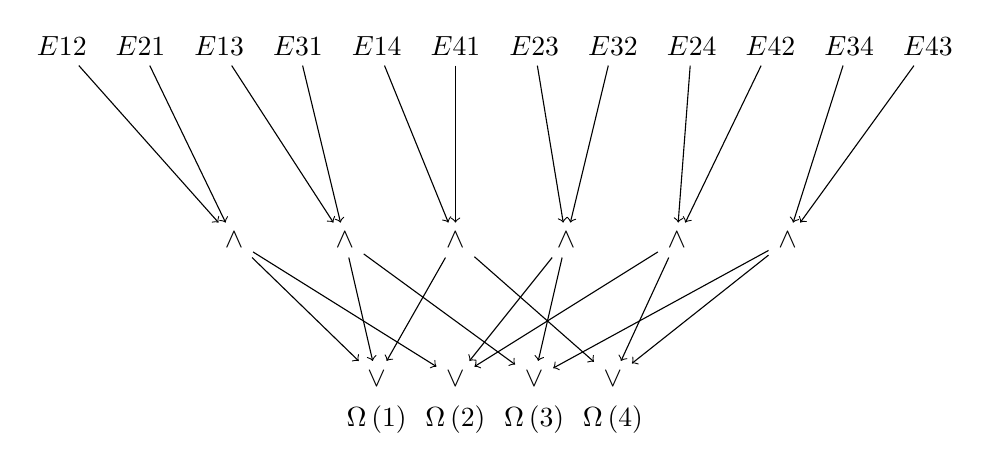
\begin{tikzpicture}

\node (E12) {$E 1 2$};
\node [right of=E12] (E21) {$E 2 1$};
\node [right of=E21] (E13) {$E 1 3$};
\node [right of=E13] (E31) {$E 3 1$};
\node [right of=E31] (E14) {$E 1 4$};
\node [right of=E14] (E41) {$E 4 1$};
\node [right of=E41] (E23) {$E 2 3$};
\node [right of=E23] (E32) {$E 3 2$};
\node [right of=E32] (E24) {$E 2 4$};
\node [right of=E24] (E42) {$E 4 2$};
\node [right of=E42] (E34) {$E 3 4$};
\node [right of=E34] (E43) {$E 4 3$};

\node [below of=E41,node distance=7em] (14) {$\wedge$};
\node [left of=14,node distance=4em] (13) {$\wedge$};
\node [left of=13,node distance=4em] (12) {$\wedge$};
\node [right of=14,node distance=4em] (23) {$\wedge$};
\node [right of=23,node distance=4em] (24) {$\wedge$};
\node [right of=24,node distance=4em] (34) {$\wedge$};

\node [below of=14,node distance=5em,label=below:$\Omega\left(2\right)$] (2) {$\vee$};
\node [left of=2,label=below:$\Omega\left(1\right)$] (1) {$\vee$};
\node [right of=2,label=below:$\Omega\left(3\right)$] (3) {$\vee$};
\node [right of=3,label=below:$\Omega\left(4\right)$] (4) {$\vee$};

\path [->]
		(E12) edge (12) (E21) edge (12)
		(E13) edge (13) (E31) edge (13)
		(E14) edge (14) (E41) edge (14)
		(E23) edge (23) (E32) edge (23)
		(E24) edge (24) (E42) edge (24)
		(E34) edge (34) (E43) edge (34)

		(12) edge (1) (12) edge (2)
		(13) edge (1) (13) edge (3)
		(14) edge (1) (14) edge (4)
		(23) edge (2) (23) edge (3)
		(24) edge (2) (24) edge (4)
		(34) edge (3) (34) edge (4)

;

\end{tikzpicture}
\par\end{centering}
\caption{\label{fig:circuit}Schaltkreis $\mathcal{C}_{4}$}
\end{figure}
\end{example*}

\section{Eigenschaften von Schaltkreisen}
\begin{defn}
\textbf{Größe und Tiefe}

Die Größe $\left|\mathcal{C}\right|$ eines Schaltkreises $\mathcal{C}=\left(G,W,\Sigma,\Omega,U\right)$
sei die Anzahl seiner Gates, $\left|G\right|$. Die Tiefe $T\left(\mathcal{C}\right)$
sei die maximale Länge eines Wegs durch den Graphen $\left(G,W\right)$.
\end{defn}

\begin{defn}
\textbf{Invarianz}

Ein $\left(\sigma,\mathbb{B}\right)$-Schaltkreis $\mathcal{C}$ mit
dem Universum $U$ heiße \textbf{invariant}, wenn für alle $\mathfrak{A}\in\mathbf{FIN}^{U}\left(\sigma\right)$,
alle $\bar{t}\in U^{\mathrm{ar}\left(\mathcal{C}\right)}$, und jede
Permutation $\pi\in\mathrm{Sym}_{U}$ gilt:
\[
\left\llbracket \mathcal{C}\right\rrbracket \left(\pi\mathfrak{A},\pi\bar{t}\right)=\left\llbracket \mathcal{C}\right\rrbracket \left(\mathfrak{A},\bar{t}\right)
\]

In diesem Fall definieren wir für jede Struktur $\mathfrak{A}\in\mathbf{FIN}^{\left(\left|U\right|\right)}\left(\sigma\right)$
und $\bar{a}\in A^{\mathrm{ar}\left(\mathcal{C}\right)}$ die Auswertung
von $\mathcal{C}$ implizit als die Auswertung auf $\pi\mathfrak{A}\in\mathbf{FIN}^{U}\left(\sigma\right)$
mit einer beliebigen Bijektion $\pi:A\rightleftarrows U$:
\[
\left\llbracket \mathcal{C}\right\rrbracket \left(\mathfrak{A},\bar{a}\right)\coloneqq\left\llbracket \mathcal{C}\right\rrbracket \left(\pi\mathfrak{A},\pi\bar{a}\right)
\]
\end{defn}

\begin{defn}
\textbf{Symmetrie}

Für einen Schaltkreis $\mathcal{C}=\left(G,W,\Sigma,\Omega,U\right)$,
eine Permutation $\pi\in\mathrm{Sym}_{U}$ und einen Automorphismus
$\rho\in\mathrm{Aut}_{\mathcal{C}}$ mit $\rho_{\mid U}=\pi$ nennen
wir $\rho$ von $\pi$ \textbf{induziert}. (Nach den formalen Definitionen
\ref{def:formal} und \ref{def:isomorphism} ist $\rho\in\mathrm{Aut}_{\mathcal{C}}\subseteq\mathrm{Sym}_{G\uplus U}$
eine Permutation des Universums von $\mathcal{C}$.) Wir können aus
der formalen Definition des Schaltkreises als $\tau_{\sigma,\mathbb{B},k}$-Struktur
ableiten, dass ein von $\pi$ induzierter Automorphismus $\rho$ die
folgenden Bedingungen erfüllt:

\begin{enumerate}
\item Die Kanten sind isomorph: $\rho W=W$.
\item Für alle Inputs $g$ mit $\Sigma\left(g\right)=R\bar{x}$ gilt $\Sigma\left(\rho g\right)=R\,\bar{x'}$,
mit $\bar{x'}=\pi\bar{x}$.
\item Für alle übrigen Gates gilt $\Sigma\left(\rho g\right)=\Sigma\left(g\right)$.
\item Für jedes Tupel $\bar{t}\in U^{k}$ gilt $\rho\Omega\left(\bar{x}\right)=\Omega\left(\pi\bar{t}\right)$.
\end{enumerate}
Ein Schaltkreis heiße \textbf{symmetrisch}, genau dann wenn jede Permutation
des Universums $\pi\in\mathrm{Sym}_{U}$ einen Automorphismus $\hat{\pi}\in\mathrm{Aut}_{\mathcal{C}}$
des Schaltkreises induziert. (In Zukunft betrachten wir der Einfachheit
halber nur den Teil $\hat{\pi}_{\mid G}$, der die Gates des Schaltkreises
permutiert, da der Rest des Automorphismus $\hat{\pi}=\hat{\pi}_{\mid G}\uplus\pi$
lediglich die Permutation $\pi$ ist.)
\end{defn}
\begin{prop}
Symmetrie ist eine hinreichende, aber nicht notwendige, Bedingung
für die Invarianz eines Schaltkreises.
\end{prop}
\begin{proof}
Sei $\mathcal{C}$ ein symmetrischer $k$-stelliger $\left(\sigma,\mathbb{B}\right)$-Schaltkreis
über $U$, und $\mathfrak{A}\in\mathbf{FIN}^{U}\left(\sigma\right)$.
Sei $\pi\in\mathrm{Sym}_{U}$ eine beliebige Permutation, und sei
$\bar{t}\in U^{k}$ ein beliebiges Tupel. Es ist zu zeigen, dass:
\begin{eqnarray*}
\left\llbracket \mathcal{C}\right\rrbracket \left(\mathfrak{A},\bar{t}\right) & = & \left\llbracket \mathcal{C}\right\rrbracket \left(\pi\mathfrak{A},\pi\bar{t}\right)
\end{eqnarray*}

Wegen der Symmetrie induziert $\pi$ einen Automorphismus $\hat{\pi}$
auf $\mathcal{C}$: 
\begin{eqnarray*}
\hat{\pi}\left(W\right) & = & W\\
\Sigma\left(\hat{\pi}g\right) & = & \begin{cases}
R\pi\bar{x} & \mathrm{f\ddot{u}r}\,\,\Sigma\left(g\right)=R\bar{x}\\
\Sigma\left(g\right) & \mathrm{sonst}
\end{cases}\\
\Omega\left(\pi\bar{x}\right) & = & \hat{\pi}\Omega\left(\bar{x}\right)\,\mathrm{f\ddot{u}r\,alle}\,\bar{x}\in U^{\mathrm{ar}\left(\mathcal{C}\right)}
\end{eqnarray*}

Per Induktion über die Tiefe\footnote{Die Tiefe $T:G\rightarrow\mathbb{N}$ sei die maximale Länge eines
Weges von einer Quelle zum Gate $g$.} $T\left(g\right)$ des Gates $g$ wird gezeigt: 
\begin{eqnarray*}
\mathcal{C}\left[\mathfrak{A}\right]\left(g\right)=\mathcal{C}\left[\pi\mathfrak{A}\right]\left(\hat{\pi}g\right) &  & \mathrm{f\ddot{u}r\,alle}\,g\in G
\end{eqnarray*}

\begin{description}
\item [{Induktionsanfang~$T\left(g\right)=0$:}] Sei $g\in G$ ein Input
mit $\Sigma\left(g\right)=R\bar{x}$. Per Definition von $\tau$ und
$\hat{\tau}$ gilt:
\begin{eqnarray*}
\Sigma\left(\hat{\pi}g\right) & = & R\pi\bar{x}\\
\pi\bar{x}\in\pi R^{\mathfrak{A}} & \Longleftrightarrow & \bar{x}\in\pi_{2}R^{\mathfrak{A}}
\end{eqnarray*}
 Es folgt: 
\begin{eqnarray*}
\mathcal{C}\left[\pi\mathfrak{A}\right]\left(\hat{\pi}g\right) & = & \left[\pi R^{\mathfrak{A}}\right]\left(\pi\bar{x}\right)\\
 & = & \left[R^{\mathfrak{A}}\right]\left(\bar{x}\right)\\
 & = & \mathcal{C}\left[\mathfrak{A}\right]\left(g\right)
\end{eqnarray*}
(Falls $\Sigma\left(g\right)\in\left\{ \mathbf{0},\mathbf{1}\right\} $,
folgt die Behauptung direkt aus $\Sigma\left(\hat{\pi}g\right)=\Sigma\left(g\right)$.)
\item [{Induktionsschritt~$n\mapsto n+1$:}] 

\begin{description}
\item [{Annahme:}] Für alle Gates $g\in G$ mit Tiefe $T\left(g\right)\leqslant n$
gilt $\mathcal{C}\left[\pi\mathfrak{A}\right]\left(\hat{\pi}g\right)=\mathcal{C}\left[\mathfrak{A}\right]\left(g\right)$.
\end{description}
So gilt für jedes Gatter $g'\in G$ mit $T\left(g'\right)=n+1$: 
\begin{enumerate}
\item Die Beschriftungen $\Sigma\left(\hat{\pi}g'\right)=\Sigma\left(g'\right)=\phi$
sind gleich.
\item $\mathcal{C}\left[\pi\mathfrak{A}\right]\left(\hat{\pi}g\right)=\mathcal{C}\left[\mathfrak{A}\right]\left(g\right)$
für alle $\left(g,g'\right)\in W$.
\end{enumerate}
Es folgt $\mathcal{C}\left[\pi\mathfrak{A}\right]\left(\hat{\pi}g'\right)=\mathcal{C}\left[\mathfrak{A}\right]\left(g'\right)$.

\end{description}
Schließlich gilt für jedes Tupel $\bar{t}\in U^{\mathrm{ar}\left(\mathcal{C}\right)}$:

\begin{eqnarray*}
\left\llbracket \mathcal{C}\right\rrbracket \left(\pi\mathfrak{A},\pi\bar{t}\right) & = & \mathcal{C}\left[\pi\mathfrak{A}\right]\left(\Omega\left(\pi\bar{t}\right)\right)\\
 & = & \mathcal{C}\left[\pi\mathfrak{A}\right]\left(\hat{\pi}\Omega\left(\bar{t}\right)\right)\\
 & = & \mathcal{C}\left[\mathfrak{A}\right]\left(\Omega\left(\bar{t}\right)\right)=\left\llbracket \mathcal{C}\right\rrbracket \left(\mathfrak{A},\bar{t}\right)
\end{eqnarray*}

Damit ist der Schaltkreis invariant.

Um die Umkehrrichtung zu widerlegen, wird als Gegenbeispiel der folgende
$0$-stellige Schaltkreis $\mathcal{C}_{2}$ (siehe Abbildung \ref{fig:symm})
über $U=\left\{ 1,2\right\} $ angeführt:
\begin{eqnarray*}
\mathcal{C} & \coloneqq & \left(G,W,\Sigma,\Omega,U\right)\\
G & \coloneqq & \left\{ g_{i,j}\mid i,j\in U\right\} \cup\left\{ g_{\wedge},g_{\wedge}'\right\} \\
W & \coloneqq & \left\{ \left(g_{1,1},g_{\wedge}\right),\left(g_{1,2},g_{\wedge}\right),\left(g_{2,1},g_{\wedge}'\right),\left(g_{2,2},g_{\wedge}'\right),\left(g_{\wedge},g_{\wedge}'\right)\right\} \\
\Sigma\left(g\right) & \coloneqq & \mathtt{AND}\\
\Omega & \coloneqq & g_{\wedge}'
\end{eqnarray*}

\begin{figure}
\begin{centering}
\begin{center}
\tikzstyle{every node}=[circle, draw=black]
\begin{tikzpicture}

\node [label=below:$\Omega$] (C) {$\wedge$};

\node [above left of=C,node distance=6em] (B1) {$\wedge$};


\node [above left of=B1,node distance=6em] (A1) {$E12$};
\node [right of=A1,node distance=5.5em] (A2) {$E11$};
\node [right of=B1,node distance=5.5em] (A3) {$E22$};
\node [right of=A3,node distance=5.5em] (A4) {$E21$};

\path [->] (A1) edge (B1) (A2) edge (B1) (A3) edge (C) (A4) edge (C)
			(B1) edge (C);
\end{tikzpicture}
\par\end{center}
\par\end{centering}
\caption{\label{fig:symm}Schaltkreis $\mathcal{C}_{2}$}
\end{figure}
\end{proof}
Der Schaltkreis ist invariant, und akzeptiert alle vollständigen $K_{2}$-Graphen.
Er ist aber nicht symmetrisch: Die Permutation $\left(\begin{array}{cc}
1 & 2\\
2 & 1
\end{array}\right)$ induziert keinen Automorphismus.

\begin{defn}
\textbf{\label{def:rigid}Rigidität}

Ein Schaltkreis $\mathcal{C}=\left(G,W,\Sigma,\Omega,U\right)$ sei
rigide, wenn er keine redundanten Gates besitzt. Formal dürfen nicht
$g,g'\in G$ existieren, so dass:
\begin{eqnarray*}
\Sigma\left(g\right) & = & \Sigma\left(g'\right)\\
\left\{ u\in G\mid\left(u,g\right)\in W\right\}  & = & \left\{ u\in G\mid\left(u,g'\right)\in W\right\} 
\end{eqnarray*}

Insbesondere heißt dies, das der Schaltkreis höchstens zwei Konstanten
$g_{0},g_{1}$ mit $\Sigma\left(g_{0}\right)=\mathbf{0}$ und $\Sigma\left(g_{1}\right)=\mathbf{1}$
enthält, und jede Input-Beschriftung $\Sigma\left(g\right)=R\bar{x}$
nur einmal vorkommt.
\end{defn}
Die Rigidität ist hier analog zu der Arbeit von Anderson und Dawar\cite{AD2014}
definiert, verlangt aber zusätzlich, dass zwei Gates nicht nur durch
die (hier nicht injektive) Output-Markierung $\Omega$ unterschieden
werden. Diese Einschränkung ist strenger, schränkt aber die Definition
nicht bedeutend ein:

Für zwei Gates $g,g'\in G$ mit den gleichen Vorgängern, der gleichen
Markierung $\Sigma\left(g\right)=\Sigma\left(g'\right)$ und $\Omega^{-1}\left(g\right)\neq\Omega^{-1}\left(g'\right)$
erlaubt die nicht-injektive Definition von $\Omega$, dass $g'$ entfernt
wird und für alle $\bar{t}\in\Omega^{-1}\left(g'\right)$ stattdessen
$\Omega\left(\bar{t}\right)\coloneqq g$ gesetzt wird.

\section{Eigenschaften von Schaltkreisfamilien}
\begin{defn}
Eine $\left(\sigma,\mathbb{B}\right)$-\textbf{Schaltkreisfamilie}
$\bar{\mathcal{C}}=\left(\mathcal{C}_{n}\right)_{n\in\mathbb{N}}$
sei eine Sequenz von invarianten Schaltkreisen $\mathcal{C}_{n}=\left(G_{n},W_{n},\Sigma_{n},\Omega_{n},U_{n}\right)$
mit der gleichen Stelligkeit $\mathrm{ar}\left(\mathcal{C}_{n}\right)=k$
und den Universen $U_{n}=\left[1,n\right]$.

Die von der Schaltkreisfamilie berechnete $\sigma$-Anfrage $q_{\bar{\mathcal{C}}}$
sei wie folgt: 
\[
q_{\bar{\mathcal{C}}}\left(\mathfrak{A}\right)\coloneqq q_{\mathcal{C}_{\left|A\right|}}\left(\mathfrak{A}\right)
\]
\end{defn}

\begin{defn}
Für eine Komplexitätsklasse $\mathcal{K}$ sei eine Schaltkreisfamilie
$\bar{\mathcal{C}}$ $\mathcal{K}$-uniform, wenn die Berechnung einer
Repräsentation von $\mathcal{C}_{n}$ bei Eingabe des Worts $\overset{n}{\overbrace{1\cdots1}}$
in $\mathcal{K}$ ist.
\end{defn}

\begin{defn}
\textbf{Beschränkte Größe}

Für eine Funktion $f:\mathbb{N}\rightarrow\mathbb{N}$ habe eine Schaltkreisfamilie
$\bar{\mathcal{C}}$ $f$-\textbf{Größe}, wenn für ein $n_{0}\in\mathbb{N}$
und alle $n\geqslant n_{0}$ gilt, dass $\left|\mathcal{C}_{n}\right|\leqslant f\left(n\right)$.
Für eine Klasse von Funktionen $\mathcal{F}\subseteq\mathrm{Abb}\left(\mathbb{N},\mathbb{N}\right)$
mit $f\in\mathcal{F}$ habe $\bar{C}$ $\mathcal{F}$-Größe.

Insbesondere sei $\mathrm{poly}\left(n\right)=n^{\mathcal{O}\left(1\right)}$
die Klasse aller polynomiell beschränkten Funktionen.
\end{defn}
\begin{rem*}
Statt ,,$\mathrm{poly}\left(n\right)$-groß`` wird in \cite{AD2014}
der Begriff ,,$\mathrm{P}/\mathrm{poly}$-uniform`` verwendet:

Eine $\mathrm{P/poly}$-Turingmaschine arbeitet in Polynomialzeit
und erhält für eine Eingabe der Länge $n$ eine polynomiell beschränkte
Orakel-Eingabe $\Upsilon\left(n\right)\in\left\{ 0,1\right\} ^{f\left(n\right)}$,
$f\left(n\right)\in\mathrm{poly}\left(n\right)$. Unter Voraussetzung
einer geeigneten Kodierung kann $\Upsilon\left(n\right)$ jede $\mathrm{poly}\left(n\right)$-große
Schaltkreisfamilie repräsentieren\cite{arora-barak}. Daher sind die
Begriffe ,,$\mathrm{poly}\left(n\right)$-groß`` und ,,$P/\mathrm{poly}$-uniform``
äquivalent.
\end{rem*}
\begin{defn}
\textbf{Beschränkte Tiefe}

Für eine Funktion $f:\mathbb{N}\rightarrow\mathbb{N}$ habe eine Schaltkreisfamilie
$\bar{\mathcal{C}}$ $f$-\textbf{Tiefe}, wenn $T\left(\mathcal{C}_{n}\right)\leqslant f\left(n\right)$
für ein $n_{0}\in\mathbb{N}$ und alle $n\geqslant n_{0}$. Für eine
Klasse $\mathcal{F}\subseteq\mathrm{Abb}\left(\mathbb{N},\mathbb{N}\right)$
sei der Begriff ,,$\mathcal{F}$-tief`` analog zu ,,$\mathcal{F}$-groß``
definiert.
\end{defn}

\begin{defn}
Benennung von Schaltkreisklassen

Sei $\sigma$ eine beliebige relationale Signatur.

\begin{itemize}
\item Mit $\mathrm{SBC}\left[\sigma\right]$ bezeichnen wir die Klasse der
Anfragen, die von einer symmetrischen\textbf{ $\left(\sigma,\mathbb{B}_{\mathrm{std}}\right)$}-Schaltkreisfamilie
beschrieben werden.
\item $\left(\mathrm{SBC}+\mathbf{MAJ}\right)\left[\sigma\right]$ sei die
Klasse der Anfragen, die von einer symmetrischen\textbf{ $\left(\sigma,\mathbb{B}_{\mathrm{maj}}\right)$}-Schaltkreisfamilie
beschrieben werden. (Zur Erinnerung: $\mathbb{B}_{\mathrm{maj}}=\mathbb{B}_{\mathrm{std}}\uplus\left\{ \mathtt{MAJ}\right\} $,
wobei $\mathtt{MAJ}$ der Majority-Operator ist.)
\end{itemize}
Für eine Komplexitätsklasse $\mathcal{K}$ bezeichne $\mathrm{SBC}^{\mathcal{K}}$
(beziehungsweise $\left(\mathrm{SBC}+\mathbf{MAJ}\right)^{\mathcal{K}}$
die Klasse der Anfragen, die von einer entsprechenden $\mathcal{K}$-uniformen
Schaltkreisfamilie beschrieben werden.

Für jede dieser Klassen schreiben wir ,,$\mathrm{SAC}^{0}$`` anstelle
von ,,$\mathrm{SBC}$``, um die Klasse auf Schaltkreisfamilien mit
konstanter Tiefe und $\mathrm{poly}\left(n\right)$-Größe zu beschränken.
\end{defn}

